% !TEX encoding = UTF-8
% !TEX TS-program = pdflatex
% !TEX root = ../tesi.tex

\chapter{ROFF}
\label{chapter:roff}

	RObust and Fast Forwarding scheme (ROFF) is a protocol proposed by Hongseok Yoo and Dongkyun Kim in \cite{6906275}. This chapter will present the two main problems tackled by ROFF already introduced in Section \ref{sec:emd}, namely the perfect suppression of redundant transmissions, which will be explained in \ref{ssec:collision-analysis} , and the disuniformity and the costant change in spatial vehicle distribution in VANETs, addressed in section \ref{ssec:latency-analysis}.

	\section{Forwarder Selection Problem}
		\subsection{Collision Analysis}
			\label{ssec:collision-analysis}
			The first problem tackled by ROFF concerns collisions caused by nodes who start to transmit at the same time. This results in a collision in the area resulting from the intersection of the nodes' transmission ranges.
			
			
			Suppose that $S_f=\{f_i | 0 < i \leq N, i \in \mathbb{N} \}$ is the set of PFCs ordered in ascending order by the distance between the previous forwarder and the PFC, where N is the number of PFCs and $f_n$ is the FFC. We define $f_0$ as the previous forwarder.
			%TODO immagine con 1..n PFC
			Based on the most common idea in existing protocols, ideally a PFC $f_i$ suppresses its scheduled transmission whenever it receives the transmission from $f_N$. In order to achieve suppression, vehicles from $f_i$ to $f_i-1$ should wait until they receive the transmission from $f_N$ before forwarding. If a vehicle forwards the message before having received the transmission from $f_N$, then a collision will occur. As stated in Section \ref{sec:emd}, existing protocols employ a strategy for waiting time assignment by which each PFC calculates its waiting time based on the distance between itself and the previous forwarder (that is $distance = d(f_i, f_0)$). As a consequence, successful suppression of all PFCs ($f_1$ to $f_{N-1}$, $f_{N-1}$ included) can be achieved only if the timer of $f_{N-1}$ is long enough to detect the transmission from $f_N$. The authors define $minDiff$ as the minimum time difference between $f_N$ and $f_{N-1}$ to prevent $f_{N-1}$ from forwarding.
			
			\begin{figure}[H]
				\centering
				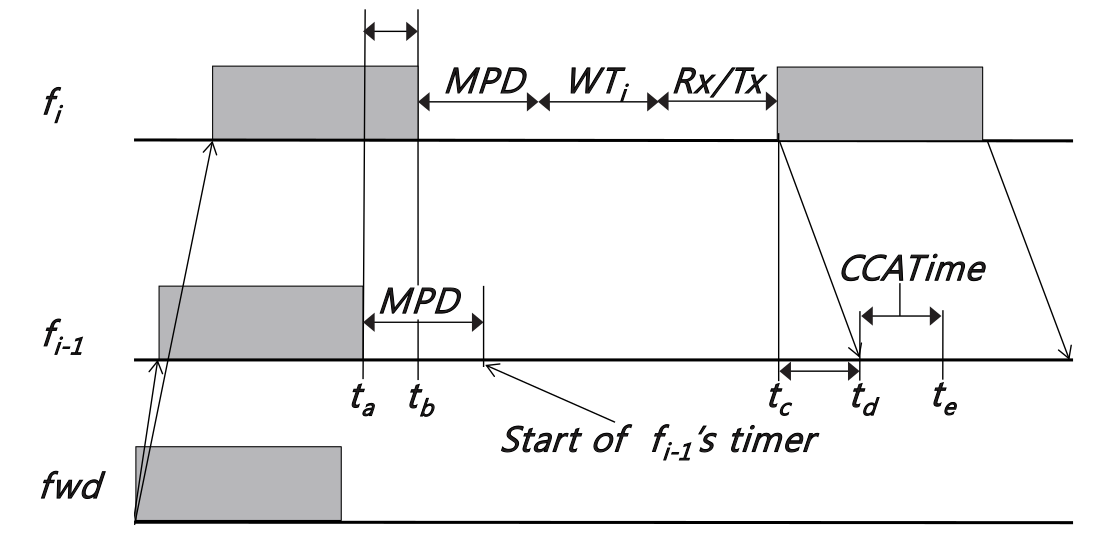
\includegraphics[width=\textwidth]{immagini/minDiff}
				\caption{Definition of $minDiff$ between $f_N$ and $f_{N-1}$ (\cite{6906275})}
				\label{fig:minDiff}
			\end{figure}
		
			\imgrefcap{fig:minDiff} depicts a situation where $fwd$ is the forwarder and $f_i$ (farther from fwd than $f_{i-1}$) relays the message before $f_{i-1}$. The two vehicles $f_i$ and $f_{i-1}$ complete receiving the message at different times ($t_a$ and $t_b$) due to propagation delay (calculated as $pd = d / s$, where $d$ is the distance between two points in space and $s$ is the wave propagation speed of the medium, i.e. $s=c$, the speed of light, in wireless communication). After reception we have additional amount of time in order to process and retransmit the message:
			\begin{itemize}
				\item Each PFC spends MAC Processing Delay (MPD) to process the message and then waits for $WT_i$ calculated according to whichever multi-hop algoritm is being used. As explained previously, this waiting time is inversely proportional to the distance between the PFC and $fwd$;
				\item After timer expiration, each PFC wait for Rx/Tx turnaround time ($Rx/Tx$), in order to switch their interface from reception to transmission mode.
			\end{itemize}
			After $f_i$ has forwarded the message, $f_{i-1}$ starts receiving it at $t_d$, $t_d-t_c$  being equal to $pd{f_{i-1}, f_i}$. The time between the PHY module of $f_{i-1}$ starts reception and the MAC module of the same vehicle is aware of reception is called $CCATime$. Hence, if $f_{i-1}$'s timer expires between $t_a$ and $t_e$, $f_{i-1}$'s transmission will collide with $f_i$'s. In order to accomplish succesful suppression, $f_{i-1}$'s timer should not expire  before $t_e$. 
			
			
			Given the fact that Propagation delay is not controllable and MPD, $Rx/Tx$ and $CCATime$ are usually standard-defined parameters, an algorithm can only manage the difference between waiting times of $f_i$ and $f_{i-1}$ (represented by $WT_i$ and $WT_{i-1}$ respectively in the following formula).
			To achieve succesful suppression, $f_{i-1}$ should wait until the forwarding from $f_i$ is detected by $f_{i-1}$ MAC layer, so $MPD+WT_{i-1}$ should be greater than $t_e - t_a$. Hence, $minDiff = (pd_{fwd, f_i} - pd_{fwd, f_{i-1}}) + pd_{f_i, f_{i-1}} + Rx/Tx + CCATime$.
		
		\subsection{Latency Analysis}
			\label{ssec:latency-analysis}
			The second problem ROFF tries to overcome is the effect of empty space in vehicle distribution on forwarding latency.
			
			The region where PFCs are placed can be defined as \textit{naive forwarding area} (NFA) and is defined as the intersection between:
			\begin{itemize}
				\item the transmission range of a forwarder $fwd$;
				\item the area in the opposite movement direction of the same forwarder $fwd$.
			\end{itemize}
			The distribution of vehicle inside NFA can vary in time; moreover, vehicles are not usually placed at the same distance, so empty spaces of various sizes exist inside the area.
			
			\begin{figure}[H]
				\centering
				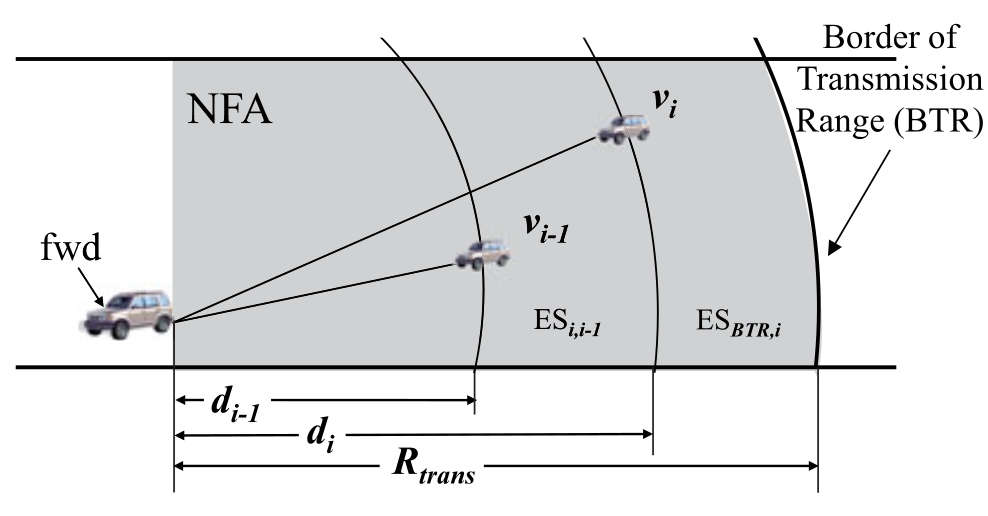
\includegraphics[width=\textwidth]{immagini/emptySpace}
				\caption{Definition of empty space (\cite{6906275})}
				\label{fig:emptySpace}
			\end{figure}
			
			Suppose that $S_v = \{v_i | 0 < i \leq M\}$ is a set of M vehicles inside NFA with vehicles ordered by distance between the vehicle and the previous forwarder in ascending order. Referring to Figure \ref{fig:emptySpace} , the empty space $ES_i,i-1$ between $v_i$ and $v_{i-1}$ is the segment within the two circles centered in $fwd$ with radius $d_{i-1}$ and $d_i$ respectively. Hence, the size of $ES_i,i-1$ is equal to $d_i - d{i-1}$.
			
			
			Large empty spaces have a negative effect on forwarding latency. There is no guarantee that the farthest vehicle from the previous forwarder become the FFC: lossy channel environments, shadowing and other phenomena can make any vehicle within NFA become the forwarder. Suppose that $fwd$ is the previous forwarder and there are two vehicles, $A$ and $B$, inside NFA where A is farther from $fwd$ than $B$, $A$ has not received the transmission from $fwd$ while B has. The empty space $ES_A,B$ between $A$ and $B$ influences the forwarding latency:
			\begin{itemize}
				\item if  $ES_A,B$ is small, $B$ relays the message after a short waiting time;
				\item if $ES_A,B$ is large, $B$ waits needlessly (since there is no other vehicle farther from $fwd$ which has received the message) a large amount of time.
			\end{itemize}
			ROFF aims at resolving the effect of empty spaces by allowing vehicles to choose waiting time inversely proportional to their \textit{unique forwarding priority} proportional to the distance between the vehicle and the previous forwarder, instead of using directly such distance in the waiting time computation.
		
	\section{ROFF Algorithm}
		The ROFF algorithm works under the following two assumptions:
		\begin{enumerate}
			\item each vehicle has access to a GPS system and a digital map;
			\item vehicles periodically (e.g. every 100 milliseconds) broadcast a Hello message containing various information, such as its position, velocity, etc. The period between each Hello message broadcast is called \textit{Beacon Interval}.
		\end{enumerate}
		The algorithm is composed of three components, as depicted in Figure \ref{fig:roffAlgo}.
	
		\begin{figure}[H]
			\centering
			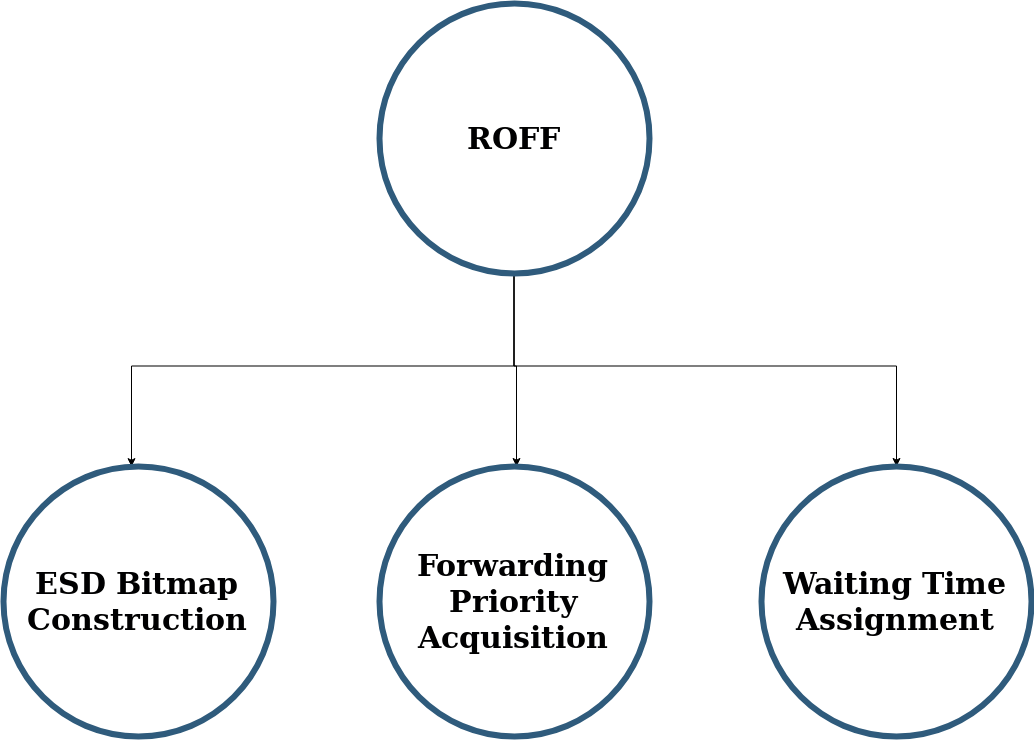
\includegraphics[width=0.7\textwidth]{immagini/roffAlgo}
			\caption{Components of ROFF algorithm}
			\label{fig:roffAlgo}
		\end{figure}
		
		
		
		
		
	